
\documentclass[tikz,border=5pt]{standalone}
\usepackage[T1]{fontenc}
\usepackage{newtxtext,newtxmath}
\usepackage{tikz}
\usetikzlibrary{arrows.meta,positioning,fit}
\definecolor{oasiblue}{RGB}{45,82,122}
\definecolor{oasigreen}{RGB}{63,108,79}
\definecolor{oasiorange}{RGB}{150,92,40}
\definecolor{oasired}{RGB}{132,54,54}
\definecolor{oasigray}{RGB}{84,91,99}
\begin{document}
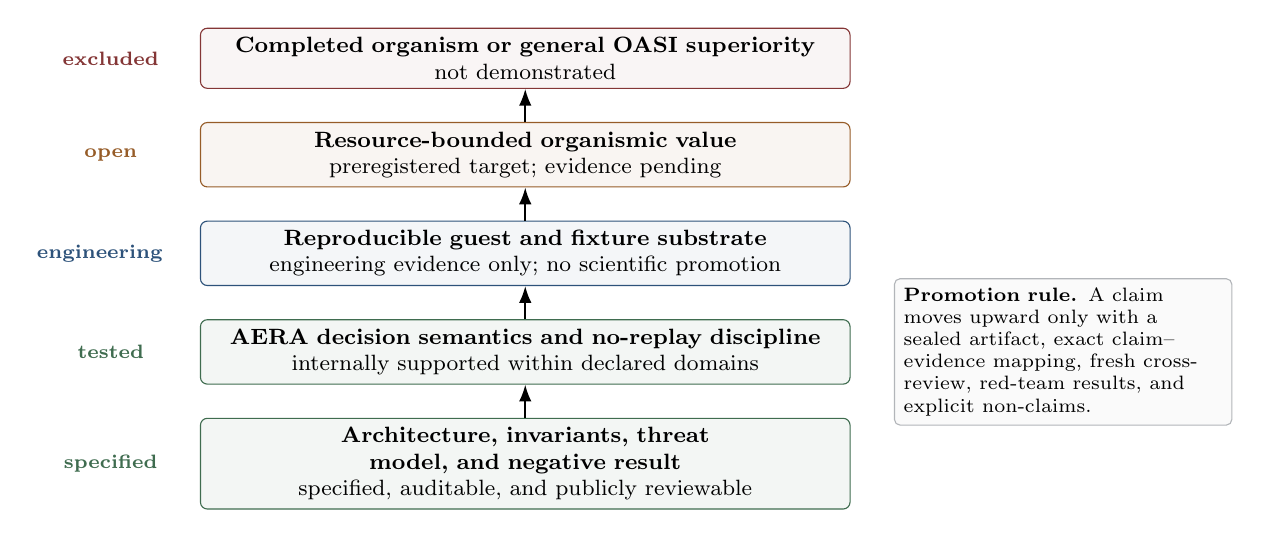
\begin{tikzpicture}[font=\footnotesize,>=Latex,
 lvl/.style={draw,rounded corners=2.5pt,minimum width=8.25cm,text width=7.9cm,
 minimum height=.66cm,align=center,fill=white},
 tag/.style={font=\scriptsize\bfseries,minimum width=1.55cm,align=center},
 arr/.style={->,line width=.68pt}]
\node[lvl,draw=oasired,fill=oasired!5] (claim)
 {\textbf{Completed organism or general OASI superiority}\\not demonstrated};
\node[lvl,draw=oasiorange,fill=oasiorange!6,below=.42cm of claim] (value)
 {\textbf{Resource-bounded organismic value}\\preregistered target; evidence pending};
\node[lvl,draw=oasiblue,fill=oasiblue!5,below=.42cm of value] (guest)
 {\textbf{Reproducible guest and fixture substrate}\\engineering evidence only; no scientific promotion};
\node[lvl,draw=oasigreen,fill=oasigreen!6,below=.42cm of guest] (aera)
 {\textbf{AERA decision semantics and no-replay discipline}\\internally supported within declared domains};
\node[lvl,draw=oasigreen,fill=oasigreen!6,below=.42cm of aera] (spec)
 {\textbf{Architecture, invariants, threat model, and negative result}\\specified, auditable, and publicly reviewable};
\draw[arr] (spec)--(aera);
\draw[arr] (aera)--(guest);
\draw[arr] (guest)--(value);
\draw[arr] (value)--(claim);

\node[tag,text=oasigreen,left=.35cm of spec] {specified};
\node[tag,text=oasigreen,left=.35cm of aera] {tested};
\node[tag,text=oasiblue,left=.35cm of guest] {engineering};
\node[tag,text=oasiorange,left=.35cm of value] {open};
\node[tag,text=oasired,left=.35cm of claim] {excluded};

\node[draw=oasigray!45,rounded corners=2pt,fill=oasigray!3,text width=4.05cm,
      align=left,font=\scriptsize,right=.55cm of aera] {
\textbf{Promotion rule.} A claim moves upward only with a sealed artifact, exact claim--evidence mapping, fresh cross-review, red-team results, and explicit non-claims.};
\end{tikzpicture}
\end{document}
